\section{Neural Networks 101}\index{neural networks}\index{neural networks!basics}
\label{sec:neural_networks_101}
% PROMPT: Showcase a minimal neural network from scratch

\subsection{Perceptrons and Multi-Layer Perceptrons (MLPs)}\index{perceptron}\index{MLP|see {Multi-Layer Perceptron}}\index{Multi-Layer Perceptron}
\begin{figure}[htbp]
\centering
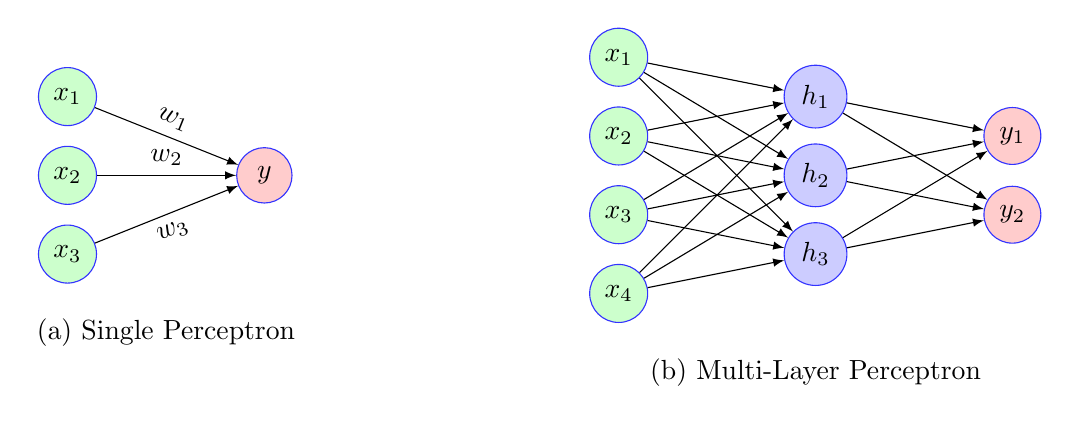
\begin{tikzpicture}[
    neuron/.style={circle, draw=blue!80, fill=blue!20, minimum size=20pt},
    input/.style={neuron, fill=green!20},
    output/.style={neuron, fill=red!20},
    >=latex
]
% Single Perceptron
\begin{scope}[xshift=-3cm]
    % Inputs
    \node[input] (x1) at (0,1) {$x_1$};
    \node[input] (x2) at (0,0) {$x_2$};
    \node[input] (x3) at (0,-1) {$x_3$};
    
    % Output neuron
    \node[output] (y) at (2.5,0) {$y$};
    
    % Connections
    \draw[->] (x1) -- node[above, sloped] {$w_1$} (y);
    \draw[->] (x2) -- node[above] {$w_2$} (y);
    \draw[->] (x3) -- node[below, sloped] {$w_3$} (y);
    
    % Title
    \node[align=center] at (1.25,-2) {(a) Single Perceptron};
\end{scope}

% Multi-Layer Perceptron
\begin{scope}[xshift=4cm]
    % Input layer
    \node[input] (i1) at (0,1.5) {$x_1$};
    \node[input] (i2) at (0,0.5) {$x_2$};
    \node[input] (i3) at (0,-0.5) {$x_3$};
    \node[input] (i4) at (0,-1.5) {$x_4$};
    
    % Hidden layer
    \node[neuron] (h1) at (2.5,1) {$h_1$};
    \node[neuron] (h2) at (2.5,0) {$h_2$};
    \node[neuron] (h3) at (2.5,-1) {$h_3$};
    
    % Output layer
    \node[output] (o1) at (5,0.5) {$y_1$};
    \node[output] (o2) at (5,-0.5) {$y_2$};
    
    % Connections for input to hidden layer
    \foreach \i in {1,2,3,4}
        \foreach \j in {1,2,3}
            \draw[->] (i\i) -- (h\j);
    
    % Connections for hidden to output layer
    \foreach \i in {1,2,3}
        \foreach \j in {1,2}
            \draw[->] (h\i) -- (o\j);
    
    % Title
    \node[align=center] at (2.5,-2.5) {(b) Multi-Layer Perceptron};
\end{scope}

\end{tikzpicture}
\caption{Neural Network Architectures\index{neural architectures}: (a) Single perceptron\index{perceptron!single} computing $y = \sigma(\sum_{i} w_i x_i + b)$\index{activation function}, where $\sigma$ is an activation function. 
(b) Multi-layer perceptron\index{perceptron!multi-layer} computing hidden layer\index{hidden layer} $h_j = \sigma(\sum_{i} w^{(1)}_{ij} x_i + b^{(1)}_j)$ followed by outputs\index{output layer} 
$y_k = \sigma(\sum_{j} w^{(2)}_{jk} h_j + b^{(2)}_k)$. This architecture enables learning complex non-linear mappings\index{non-linear mappings} through multiple layers of transformation\index{transformation layers}.}
\label{fig:neural_architectures}
\end{figure}

\noindent
Neural networks\index{neural networks!definition} have revolutionized modern machine learning\index{machine learning} by learning \emph{non-linear}\index{non-linear} mappings from input features\index{input features} to output predictions\index{output predictions} without the need for manually engineered features\index{feature engineering}. In the context of language modeling\index{language modeling}, neural networks are particularly powerful because they can encode and combine linguistic features\index{linguistic features} in high-dimensional spaces\index{high-dimensional spaces}, capturing nuances that simpler statistical models\index{statistical models} may overlook.

\noindent
The \textbf{perceptron} (Figure~\ref{fig:neural_architectures}), introduced by Frank Rosenblatt in the late 1950s, is one of the earliest forms of a trainable neural network. It models a single neuron with:
\begin{enumerate}
    \item A set of input weights.
    \item A linear combination of inputs and weights.
    \item A non-linear activation function (e.g., step function).
\end{enumerate}
While a single perceptron can only represent linear decision boundaries, stacking multiple perceptrons in layers (known as a \textbf{Multi-Layer Perceptron}, or MLP) allows for the modeling of highly complex, non-linear relationships.

\begin{itemize}
    \item \textbf{Input Layer.} Receives the raw features, such as token embeddings in NLP.
    \item \textbf{Hidden Layers.} Non-linear transformations are applied in each layer. Common activation functions include $\text{ReLU}, \tanh, \text{sigmoid}$.
    \item \textbf{Output Layer.} Produces the final prediction, such as a probability distribution over the next token for language modeling.
\end{itemize}

\subsection{Forward and Backpropagation}\index{forward propagation}\index{backpropagation}
\noindent
Learning in neural networks typically involves two main steps:
\begin{itemize}
    \item \textbf{Forward Propagation.} The process of moving data through the network from input to output:
    
    \begin{itemize}
        \item \textbf{Input Layer Processing:}
            \begin{itemize}
                \item Raw input features enter the network
                \item Each feature is weighted according to learned parameters
                \item The weighted inputs are combined and passed through an activation function
            \end{itemize}
            
        \item \textbf{Hidden Layer Transformations:}
            \begin{itemize}
                \item Each hidden layer receives processed information from the previous layer
                \item The network learns increasingly complex representations at each layer
                \item Non-linear activation functions allow the network to model complex patterns
                \item Each neuron acts as a feature detector, learning to recognize specific patterns
            \end{itemize}
            
        \item \textbf{Output Layer Generation:}
            \begin{itemize}
                \item The final layer produces predictions based on all previous transformations
                \item Output format depends on the task (e.g., probabilities for classification)
                \item The network's prediction is compared to the true target to compute error
            \end{itemize}
            
        \item \textbf{Key Concepts:}
            \begin{itemize}
                \item Information flows in one direction: input → hidden layers → output
                \item Each connection has a weight that's learned during training
                \item Bias terms allow the network to shift activation functions
                \item The network builds a hierarchical representation of the input data
            \end{itemize}
    \end{itemize}
    
    \begin{equation}\label{eq:forward_prop}
        \mathbf{z}^{(l)} = \mathbf{W}^{(l)} \mathbf{h}^{(l-1)} + \mathbf{b}^{(l)}, \quad \mathbf{h}^{(l)} = \sigma(\mathbf{z}^{(l)})
    \end{equation}
    where $\sigma(\cdot)$ is a non-linear activation function\index{activation function}, and $\mathbf{h}^{(0)} \equiv \mathbf{x}$ is the input vector\index{input vector}.

    \item \textbf{Backward Propagation (Backprop).}\index{backpropagation!definition} The backbone of neural network training\index{training}, backpropagation enables neural networks to learn from their mistakes through:
    \begin{itemize}
        \item \textbf{Error Attribution:}
            \begin{itemize}
                \item Determines how much each neuron contributed to the network's error
                \item Traces the path of mistakes backwards through the network
                \item Identifies which weights need the most adjustment
                \item Helps understand which parts of the network are most responsible for incorrect predictions
            \end{itemize}
            
        \item \textbf{Learning Process:}
            \begin{itemize}
                \item Adjusts weights to minimize prediction errors
                \item Stronger corrections for neurons that contributed more to mistakes
                \item Weaker corrections for neurons that had less impact
                \item Balances the influence of different network components
            \end{itemize}
            
        \item \textbf{Optimization Benefits:}
            \begin{itemize}
                \item Efficiently updates millions of parameters simultaneously
                \item Prevents the need for trial-and-error weight adjustment
                \item Enables deep networks to learn complex patterns
                \item Provides a systematic way to improve network performance
            \end{itemize}
            
        \item \textbf{Training Insights:}
            \begin{itemize}
                \item Helps identify learning problems (e.g., vanishing gradients)
                \item Guides the choice of learning rates and optimization strategies
                \item Indicates which parts of the network are learning effectively
                \item Assists in debugging network architectures
            \end{itemize}
    \end{itemize}

    \begin{itemize}
        \item \textbf{Chain Rule Application:} For a composite function $f(g(x))$, the chain rule states:
        \begin{equation}
            \frac{\partial f(g(x))}{\partial x} = \frac{\partial f}{\partial g} \cdot \frac{\partial g}{\partial x}
        \end{equation}
        
        \item \textbf{Gradient Flow:}\index{gradient flow} Starting from the output layer\index{output layer} and moving backward:
        \begin{enumerate}
            \item Compute loss gradient\index{loss gradient}: $\frac{\partial \mathcal{L}}{\partial \hat{\mathbf{y}}}$
            \item For each layer $l$, compute:
                \begin{align}
                    \frac{\partial \mathcal{L}}{\partial \mathbf{z}^{(l)}} &= \frac{\partial \mathcal{L}}{\partial \mathbf{h}^{(l)}} \cdot \frac{\partial \mathbf{h}^{(l)}}{\partial \mathbf{z}^{(l)}} \\
                    \frac{\partial \mathcal{L}}{\partial \mathbf{W}^{(l)}} &= \frac{\partial \mathcal{L}}{\partial \mathbf{z}^{(l)}} \cdot \frac{\partial \mathbf{z}^{(l)}}{\partial \mathbf{W}^{(l)}}
                \end{align}
        \end{enumerate}
        
        \item \textbf{Parameter Updates:} Using computed gradients, parameters are updated:
        \begin{equation}
            \mathbf{W}^{(l)} \leftarrow \mathbf{W}^{(l)} - \alpha \frac{\partial \mathcal{L}}{\partial \mathbf{W}^{(l)}}
        \end{equation}
        where $\alpha$ is the learning rate.
    \end{itemize}

    Modern deep learning frameworks like PyTorch and TensorFlow implement automatic differentiation, computing these gradients efficiently without manual derivation. However, understanding the underlying mathematics remains crucial for:
    \begin{itemize}
        \item Debugging training issues
        \item Implementing custom layers
        \item Optimizing network architectures
        \item Choosing appropriate learning rates and optimization strategies
    \end{itemize}


    The learning rate $\alpha$ is a crucial hyperparameter that controls how large steps we take during training. A large learning rate means taking bigger steps, potentially learning faster but risking overshooting the optimal solution. A small learning rate takes smaller, more careful steps, leading to more stable training but requiring more time to converge. Finding the right learning rate is often a balancing act: too large and the training might diverge, too small and the training might be impractically slow or get stuck in local minima.
\end{itemize}


This loop of forward and backward propagation, repeated over multiple \emph{epochs} of training data, enables a neural network to \emph{learn} complex transformations—an essential capability for tasks like language modeling.

\noindent
An epoch represents one complete pass through the entire training dataset. During each epoch:
\begin{itemize}
    \item Every training example is used once for forward propagation
    \item The network's predictions are compared with true values
    \item Weights are updated through backpropagation
    \item The process is repeated for multiple epochs until the network converges
\end{itemize}

\noindent
Training typically requires multiple epochs because:
\begin{itemize}
    \item The network needs repeated exposure to learn complex patterns
    \item Initial weight updates may be suboptimal
    \item Different aspects of the data may be learned in different epochs
    \item The learning process is iterative and gradual
\end{itemize}

\subsection{Activation Functions}
\noindent
Activation functions impart non-linearity, allowing neural networks to model non-trivial functions. Without activation functions, neural networks would be limited to linear transformations, regardless of their depth. Here's why they're essential:

\begin{itemize}
    \item \textbf{Non-linearity:} Real-world problems rarely follow linear patterns. Activation functions enable networks to learn and represent complex, non-linear relationships in data.
    
    \item \textbf{Feature Transformation:} Each neuron can learn to activate for different input patterns, effectively becoming specialized feature detectors.
    
    \item \textbf{Gradient Flow:} Different activation functions affect how gradients flow through the network during training, influencing learning dynamics.
    
    \item \textbf{Output Range:} Activation functions can bound outputs to specific ranges (e.g., [0,1] for sigmoid, [-1,1] for tanh), which is useful for tasks like probability prediction.
\end{itemize}

See Figure \ref{fig:activation_functions} for a comparison of common activation functions.

\begin{figure}[h]
\centering
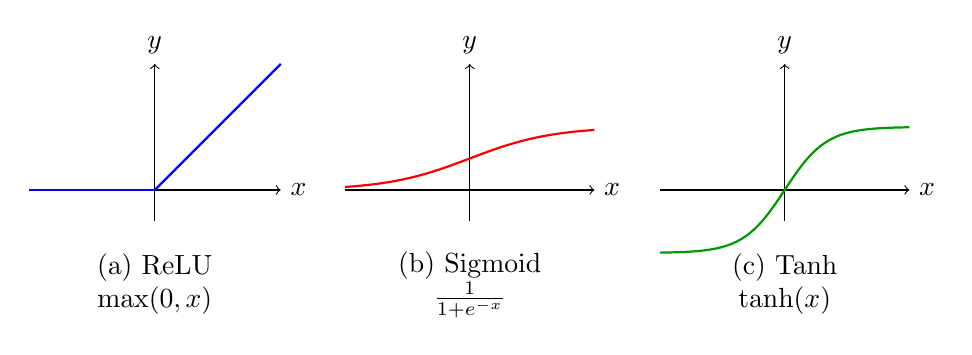
\begin{tikzpicture}[
    declare function={
        relu(\x) = max(0,\x);
        sigmoid(\x) = 1/(1 + exp(-\x));
        tanhy(\x) = (exp(\x) - exp(-\x))/(exp(\x) + exp(-\x));
    },
    scale=0.8
]
% Grid and axes for ReLU
\begin{scope}[xshift=-5cm]
    \draw[->] (-2,0) -- (2,0) node[right] {$x$};
    \draw[->] (0,-0.5) -- (0,2) node[above] {$y$};
    \draw[thick, blue] (-2,0) -- (0,0);
    \draw[thick, blue] (0,0) -- (2,2);
    \node[align=center] at (0,-1.5) {(a) ReLU\\$\max(0,x)$};
\end{scope}

% Grid and axes for Sigmoid
\begin{scope}[xshift=0cm, xscale=0.66]
    \draw[->] (-3,0) -- (3,0) node[right] {$x$};
    \draw[->] (0,-0.5) -- (0,2) node[above] {$y$};
    \draw[thick, red, domain=-3:3, samples=100] 
        plot (\x,{sigmoid(\x)});
    \node[align=center] at (0,-1.5) {(b) Sigmoid\\$\frac{1}{1+e^{-x}}$};
\end{scope}

% Grid and axes for Tanh
\begin{scope}[xshift=5cm, xscale=0.66]
    \draw[->] (-3,0) -- (3,0) node[right] {$x$};
    \draw[->] (0,-0.5) -- (0,2) node[above] {$y$};
    \draw[thick, green!60!black, domain=-3:3, samples=100] 
        plot (\x,{tanhy(\x)});
    \node[align=center] at (0,-1.5) {(c) Tanh\\$\tanh(x)$};
\end{scope}

\end{tikzpicture}
\caption{Common activation functions used in neural networks: (a) ReLU is simple and effective but suffers from the dying ReLU problem, (b) Sigmoid maps to $(0,1)$ but can saturate, (c) Tanh maps to $(-1,1)$ with stronger gradients near zero compared to sigmoid.}
\label{fig:activation_functions}
\end{figure}

\begin{itemize}
    \item \textbf{ReLU (Rectified Linear Unit):} 
    \begin{equation}\label{eq:relu}
        \sigma(z) = \max(0, z)
    \end{equation}
    Efficient and popular, though it can cause `dying ReLU' issues.
    
    \item \textbf{Sigmoid:}\index{sigmoid}\index{activation functions!sigmoid} 
    \begin{equation}\label{eq:sigmoid}
        \sigma(z) = \frac{1}{1+e^{-z}}
    \end{equation}
    Outputs values in $(0,1)$, but can saturate for large $|z|$.
    
    \item \textbf{Tanh:}\index{tanh}\index{activation functions!tanh} 
    \begin{equation}\label{eq:tanh}
        \sigma(z) = \tanh(z) = \frac{e^z - e^{-z}}{e^z + e^{-z}}
    \end{equation}
    A shifted and scaled version of the sigmoid function, outputs values in $(-1, 1)$. Also prone to saturation.
\end{itemize}

\subsection{Minimal Neural Network Example}
\noindent
The following code is a minimal example in Python of a single hidden-layer neural network for a binary classification task:

\begin{pythoncode}[Minimal Neural Network Example]
    import numpy as np
    import torch
    import torch.nn as nn
    from torch.utils.data import DataLoader
    
    # Part 1: Network Architecture and Initialization
    # ---------------------------------------------
    input_size = D
    hidden_size = H
    output_size = 1  # for binary classification
    
    # Initialize parameters
    W1 = np.random.normal(0, 0.01, (D, H))  # or torch.randn for PyTorch
    b1 = np.zeros(H)
    W2 = np.random.normal(0, 0.01, (H, output_size))
    b2 = np.zeros(output_size)
    
    
    # Part 2: Forward Pass Implementation
    # ---------------------------------
    def forward(x):
        # First layer
        z1 = x @ W1 + b1
        h1 = np.maximum(0, z1)  # ReLU activation
        
        # Output layer
        z2 = h1 @ W2 + b2
        y_pred = 1 / (1 + np.exp(-z2))  # sigmoid activation
        
        return y_pred, (z1, h1, z2)  # Return activations for backprop
    
    
    # Part 3: Backpropagation Implementation
    # ------------------------------------
    def compute_gradients(loss, y_pred, cache, x, y_true):
        z1, h1, z2 = cache
        
        # Gradient of loss with respect to output
        dy_pred = (y_pred - y_true) / len(y_true)
        
        # Gradients for output layer
        dz2 = dy_pred * y_pred * (1 - y_pred)  # sigmoid derivative
        dW2 = h1.T @ dz2
        db2 = np.sum(dz2, axis=0)
        
        # Gradients for hidden layer
        dh1 = dz2 @ W2.T
        dz1 = dh1 * (z1 > 0)  # ReLU derivative
        dW1 = x.T @ dz1
        db1 = np.sum(dz1, axis=0)
        
        return {'W1': dW1, 'b1': db1, 'W2': dW2, 'b2': db2}
    
    
    # Part 4: Training Loop
    # -------------------
    learning_rate = 0.01
    
    for epoch in range(num_epochs):
        for x_batch, y_batch in data_loader:
            # Forward pass
            y_pred, cache = forward(x_batch)
            
            # Compute binary cross-entropy loss
            loss = -np.mean(
                y_batch * np.log(y_pred) + 
                (1 - y_batch) * np.log(1 - y_pred)
            )
            
            # Compute gradients
            grads = compute_gradients(loss, y_pred, cache, x_batch, y_batch)
            
            # Update parameters
            W1 -= learning_rate * grads['W1']
            b1 -= learning_rate * grads['b1']
            W2 -= learning_rate * grads['W2']
            b2 -= learning_rate * grads['b2']
    \end{pythoncode}

\noindent
While this example is basic, the core ideas of forward propagation, loss computation, and backpropagation remain the same in more advanced architectures used in modern NLP tasks.

\subsection{Optimization Challenges}
\noindent
Despite their remarkable flexibility, neural networks are not without pitfalls. Common optimization challenges include:
\begin{itemize}
    \item \textbf{Vanishing/Exploding Gradients.} Deeper networks or RNNs may run into gradient magnitudes that become either too small or too large, slowing or destabilizing training.
    \item \textbf{Overfitting.} A network with many parameters can easily memorize the training data. Techniques such as \emph{dropout}, \emph{weight decay}, and \emph{batch normalization} help mitigate overfitting.
    \item \textbf{Choosing Hyperparameters.} Finding the right learning rate, batch size, and network architecture often involves empirical experimentation.
\end{itemize}

\noindent
Understanding these fundamental concepts is crucial before diving into more specialized architectures, such as Transformers. By grounding ourselves in the mechanics of standard neural networks, we lay the foundation for comprehending how modern LLMs leverage and extend these principles to handle vast amounts of textual data at massive scales.

\section{Overfitting and Regularization}\index{overfitting}\index{regularization}
\label{sec:overfitting_regularization}

\noindent
In the context of Large Language Models\index{LLM!overfitting}, overfitting occurs when a model performs well on training data\index{training data} but fails to generalize\index{generalization} to unseen examples. This section explores common regularization techniques\index{regularization techniques} used to combat overfitting in neural networks\index{neural networks!regularization}, with particular attention to their application in transformer-based architectures\index{transformer!regularization}.

\subsection{Understanding Overfitting}\index{overfitting!understanding}
\noindent
Overfitting manifests when a model learns to:
\begin{itemize}
    \item Memorize training examples\index{memorization} rather than learning generalizable patterns\index{patterns!generalizable}
    \item Capture noise\index{noise} in the training data rather than underlying relationships\index{relationships!underlying}
    \item Perform significantly better on training data than validation data\index{validation data}, showing a large generalization gap\index{generalization gap}
\end{itemize}

\subsection{Common Regularization Techniques}\index{regularization!techniques}

\subsubsection{Dropout}\index{dropout}
\noindent
Dropout\index{dropout!mechanism} randomly deactivates neurons during training with probability $p$, forcing the network to learn redundant representations\index{redundant representations}:

\begin{equation}
\mathbf{h}_\text{dropout} = \mathbf{m} \odot \mathbf{h}, \quad \mathbf{m}_i \sim \text{Bernoulli}(p)
\end{equation}

where $\odot$ represents element-wise multiplication\index{element-wise multiplication}, and $\mathbf{m}$ is the dropout mask\index{dropout!mask}.

Key benefits include:
\begin{itemize}
    \item Prevents co-adaptation\index{co-adaptation} of neurons
    \item Acts as implicit model ensemble\index{model ensemble}
    \item Reduces overfitting without increasing computational cost\index{computational cost}
\end{itemize}

\subsubsection{Weight Decay (L2 Regularization)}\index{weight decay}\index{L2 regularization}
\noindent
Weight decay\index{weight decay!mechanism} adds a penalty term to the loss function\index{loss function} based on the magnitude of weights:

\begin{equation}
\mathcal{L}_\text{total} = \mathcal{L}_\text{original} + \lambda \sum_{w \in \text{weights}} \|w\|^2
\end{equation}

where $\lambda$\index{regularization strength} controls the strength of regularization. This technique:
\begin{itemize}
    \item Encourages smaller weight values\index{weight values}
    \item Promotes smoother model behavior\index{model behavior}
    \item Helps prevent extreme parameter values\index{parameter values}
\end{itemize}

\subsubsection{Early Stopping}\index{early stopping}
\noindent
Early stopping\index{early stopping!mechanism} monitors validation performance\index{validation performance} and stops training when performance begins to degrade:
\begin{itemize}
    \item Tracks validation metrics\index{validation metrics} across epochs\index{epochs}
    \item Implements patience\index{early stopping!patience} to avoid stopping too early
    \item Saves best model checkpoint\index{model checkpoint} based on validation performance
\end{itemize}

\subsection{Transformer-Specific Regularization}\index{transformer!regularization}

\subsubsection{Attention Dropout}\index{attention dropout}
\noindent
In transformer architectures\index{transformer!architecture}, dropout is applied at multiple locations:
\begin{itemize}
    \item Attention weights dropout\index{attention!weights dropout}
    \item Hidden state dropout\index{hidden state dropout}
    \item Feed-forward layer dropout\index{feed-forward dropout}
\end{itemize}

\subsubsection{Layer Normalization}\index{layer normalization}
\noindent
Layer normalization\index{layer normalization!mechanism} helps stabilize training by normalizing activations\index{activation normalization}:

\begin{equation}
\text{LayerNorm}(x) = \gamma \odot \frac{x - \mu}{\sqrt{\sigma^2 + \epsilon}} + \beta
\end{equation}

where $\gamma$ and $\beta$ are learnable parameters\index{learnable parameters}, and $\epsilon$ is a small constant for numerical stability\index{numerical stability}.

\subsection{Practical Considerations}\index{practical considerations}

\noindent
When implementing regularization techniques\index{regularization!implementation}, consider:
\begin{itemize}
    \item \textbf{Hyperparameter Selection:}\index{hyperparameter selection}
    \begin{itemize}
        \item Dropout rate\index{dropout!rate} (typically 0.1-0.5)
        \item Weight decay coefficient\index{weight decay!coefficient}
        \item Early stopping patience\index{patience}
    \end{itemize}
    
    \item \textbf{Monitoring:}\index{monitoring}
    \begin{itemize}
        \item Training vs. validation curves\index{learning curves}
        \item Parameter magnitude distributions\index{parameter distributions}
        \item Gradient statistics\index{gradient statistics}
    \end{itemize}
    
    \item \textbf{Combination Effects:}\index{regularization!combinations}
    \begin{itemize}
        \item Different techniques may interact\index{technique interactions}
        \item Need to balance multiple regularization methods\index{regularization balance}
        \item Consider computational overhead\index{computational overhead}
    \end{itemize}
\end{itemize}

\noindent
Effective regularization\index{regularization!effective} is crucial for training robust language models\index{language models!robustness} that generalize well to unseen data\index{generalization!unseen data} while maintaining computational efficiency\index{computational efficiency}.

